%%%%%%%%%%%%%%%%%%%%%%%%%%%%%%%%%%%%%%%%%
%	
%	Clusters particionais com dados numéricos
% 	The Elbow Method
%  	Versão: 30/03/2020
%
% 	Autores:
%	 
%	 
%
%%%%%%%%%%%%%%%%%%%%%%%%%%%%%%%%%%%%%%%%%

%----------------------------------------------------------------------------------------
%	PACKAGES AND OTHER DOCUMENT CONFIGURATIONS
%----------------------------------------------------------------------------------------

\documentclass[12pt, a4paper, oneside]{scrreport}
\usepackage[T1]{fontenc}
\usepackage{wrapfig}
\usepackage[portuguese]{babel} 
\usepackage{graphicx}
\usepackage{amsmath}
\usepackage{amsfonts}
\usepackage{multicol}
\usepackage{setspace}
\usepackage[hyphens]{url}
\usepackage{utopia}
\usepackage{hyperref}
\usepackage[dvipsnames]{xcolor}
%\usepackage{fancyhdr}
\usepackage{libertine}
\usepackage{blindtext}
\usepackage[plainfootsepline]{scrlayer-scrpage}
\usepackage{listings}
\usepackage{caption}
\usepackage{subcaption}
\usepackage{enumitem}

%-------------------------------------------------------------------------------
%	SPECIFIC CONFIGURATIONS 
%---------------------------------------------------------------------
 
%pagestyle
 
 

%MULTICOL

\setlength{\columnsep}{1cm}

%INCLUDEGRAPHICS

\graphicspath{{Figures/}} %Pasta de input de imagens, gráficos, ...

%HYPERREF
\hypersetup{
	colorlinks=true,
	linkcolor=black,
	urlcolor=black,
    urlbordercolor=black,
    linkbordercolor=white,
    pdfborderstyle={/S/U/W 1},
    pdftitle={The Elbow Method},
    pdfpagemode=FullScreen
}

\makeatletter
\Hy@AtBeginDocument{%
  \def\@pdfborder{0 0 1}% Overrides border definition set with colorlinks=true
  \def\@pdfborderstyle{/S/U/W 1}% Overrides border style set with colorlinks=true
                                % Hyperlink border style will be underline of width 1pt
}
\makeatother

%CAPTIONS

\DeclareCaptionType{myequation}[][Lista de Equações]
\captionsetup[myequation]{labelformat=empty}


%-------------------------------------------------------------------------------
%	Colors
%-------------------------------------------------------------------------------

\definecolor{uminho}{RGB}{125,58,64}


%-------------------------------------------------------------------------------
%	Chapter Style
%-------------------------------------------------------------------------------
\RedeclareSectionCommand[
  beforeskip=1sp minus 1sp,
  font=\Huge\fontfamily{put}\color{white}
]{chapter}

\renewcommand\chapterformat{%
  \makebox[0pt][r]{\Huge{\thechapter}\enskip
    \textcolor{white}{\smash{\rule[-0.5\dp\strutbox]{3pt}{1cm}}}%
}}

\newlength\chapterleftmargin
\newcommand\chaptervmargin{1.5em}

\makeatletter
\renewcommand\chapterlinesformat[3]{%
  \vspace*{\dimexpr-1in-\headsep-\headheight-\topmargin-1ex}%
  \Ifthispageodd
    {\setlength\chapterleftmargin{\dimexpr1in+\hoffset+\oddsidemargin\relax}}
    {\setlength\chapterleftmargin{\dimexpr\paperwidth-\textwidth-1in-\hoffset-\oddsidemargin\relax}}
    \hspace*{-\chapterleftmargin}%
    \makebox[0pt][l]{%
      \colorbox{uminho}{%
        \parbox[t][\dimexpr\totalheight+\chaptervmargin*2\relax][c]{\dimexpr\paperwidth-2\fboxsep\relax}{%
          \makebox[\dimexpr\chapterleftmargin-\fboxsep\relax][r]{#2}%
          \Ifstr{#2}{}
            {\parbox[t]{\textwidth}{\raggedchapter#3}}
            {\enskip\parbox[t]{\dimexpr\textwidth-.5em\relax}{\raggedchapter#3}}%
        }%
      }%
    }%
}
\makeatother
%-------------------------------------------------------------------------------
%	Section Style
%-------------------------------------------------------------------------------
\def\chpcolor{uminho}
\def\chpcolortxt{uminho}
\def\sectionfont{\Large\fontfamily{put}\selectfont}

\setcounter{secnumdepth}{2}

\makeatletter

\def\@sectionstrut{\vrule\@width\z@\@height12.5\p@}
\def\@makesectionhead#1{%
  {\par%
    \raggedleft\sectionfont
   \colorbox{\chpcolor}{%
     \parbox[t]{90pt}{\color{white}\@sectionstrut\@depth4.5\p@\hfill
       \ifnum\c@secnumdepth>\z@\thesection\fi}%
   }%
   \begin{minipage}[t]{\dimexpr\textwidth-90pt-2\fboxsep\relax}
   \color{\chpcolortxt}\@sectionstrut\hspace{5pt}#1
   \end{minipage}\par
   \vspace{10pt}%
  }
}
\def\section{\@afterindentfalse\secdef\@section\@ssection}
\def\@section[#1]#2{%
  \ifnum\c@secnumdepth>\m@ne
    \refstepcounter{section}%
    \addcontentsline{toc}{section}{\protect\numberline{\thesection}#1}%
  \else
    \phantomsection
    \addcontentsline{toc}{section}{#1}%
  \fi
  \sectionmark{#1}%
  \if@twocolumn
    \@topnewpage[\@makesectionhead{#2}]%
  \else
    \@makesectionhead{#2}\@afterheading
  \fi
}
\def\@ssection#1{%
  \if@twocolumn
    \@topnewpage[\@makesectionhead{#1}]%
  \else
    \@makesectionhead{#1}\@afterheading
  \fi
}
\makeatother
%----------------------------------------------------------------------------------------
%	Subsection Style
%----------------------------------------------------------------------------------------
\setkomafont{subsection}{\color{uminho}\Large\fbox}
 
%----------------------------------------------------------------------------------------
%	TITLE SECTION
%----------------------------------------------------------------------------------------

\begin{document}

\renewcommand{\normalfont}{\fontfamily{phv}\selectfont} %font tem de estar dentro de document
\normalfont

\clearpairofpagestyles



\pagenumbering{arabic} 

\begin{flushleft}

\includegraphics[scale = 0.075]{Minho_University.png}
 \large{\\Universidade do Minho\\\normalsize{\today}}
\end{flushleft}
\rule{\textwidth}{0.5pt}
\begin{flushright}
\Huge{\textbf{O Método \textit{Elbow}}} \\ {\Large Clusters particionais com dados numéricos}
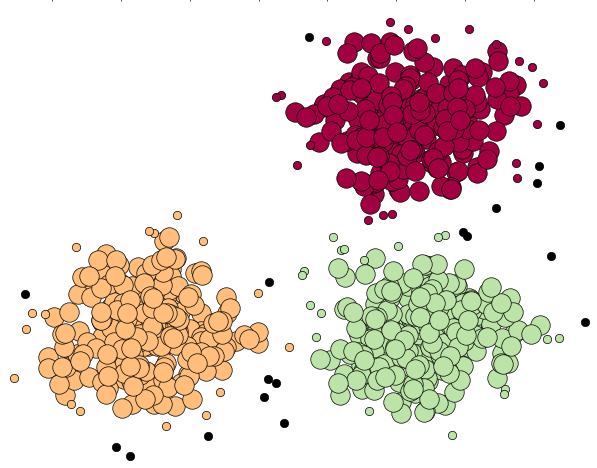
\includegraphics[scale = 0.55]{Cluster-Segmentation.png}
\end{flushright}

\begin{center}
\rule{\textwidth}{0.5pt}
\end{center}
\begin{multicols*}{2}
\noindent
\large Bruno Jácome, A89515\\
  Carolina Barros, A84950\\
  Dinis Gomes, A87993\\
  Joana Gouveia, A85650\columnbreak
  \\João Silva, A84617\\
  Jorge Gonçalves, A84133\\
  Pedro Peixoto, A89602
\end{multicols*}

%----------------------------------------------------------------------------------------
%	Índice
%----------------------------------------------------------------------------------------
\setstretch{1.5}

\renewcommand*\contentsname{Índice}
\tableofcontents

\renewcommand{\listfigurename}{Lista de Ilustrações}
\listoffigures

\renewcommand{\listtablename}{Tabelas}
\listoftables

%----------------------------------------------------------------------------------------
%	ABSTRACT AND KEYWORDS
%----------------------------------------------------------------------------------------
\newpage

\setlength{\leftmargini}{-0,35cm}
\setlength{\leftmarginii}{-0,35cm}
\setstretch{1.5}

\renewcommand{\chaptermark}[1]{\markboth{#1}{}}
\ifoot*{\color{gray}Universidade do Minho}
\ofoot*{\color{gray} \leftmark\hspace{0.25cm}|\hspace{0.25cm}\thepage}


\renewcommand{\abstractname}{Sumário} 

%Sumário se quisermos

%----------------------------------------------------------------------------------------
%	Introdução
%----------------------------------------------------------------------------------------
\chapter{Introdução}

%Retirar palha e tentar tirar coisas para meter no sumário


Este trabalho foi realizado no âmbito da Unidade Curricular de Matemática das Coisas e tem como objetivo primordial o estudo do \textit{Clusters} particionais com dados numéricos (centróide) atráves do  \textit{The Elbow Method}.\par
O presente relatório divide-se essencialmente em 4 partes. Primeiramente, no Capítulo 2, será feita uma contextualização do assunto, apresentan-se a definição de clusters no geral e, mais em concreto, de clusters particionais.\par
Seguidamente, no Capítulo 3, será descrito o conceito de centróides, bem como outros aspetos relevantes relativos.\par
Depois, no Capítulo 4, será abordado o \textit{The Elbow Method}, com a apresentação da definição teórica e a sua aplicação mais prática.\par
No capítulo seguinte, a parte teórica será aplicada em exemplos mais práticos, de forma a melhor entendermos a aplicação dos tópicos referidos nos capítulos anteriores.\par 
Para finalizar, expor-se-á uma breve conclusão do trabalho apontando-se os aspetos mais enriquecedores para o nosso conhecimento.

%----------------------------------------------------------------------------------------
%	Definição de clusters 
%----------------------------------------------------------------------------------------
\newpage

\chapter{Clusters}
\section{O que são?}
\begin{wrapfigure}{r}{0.45\textwidth}
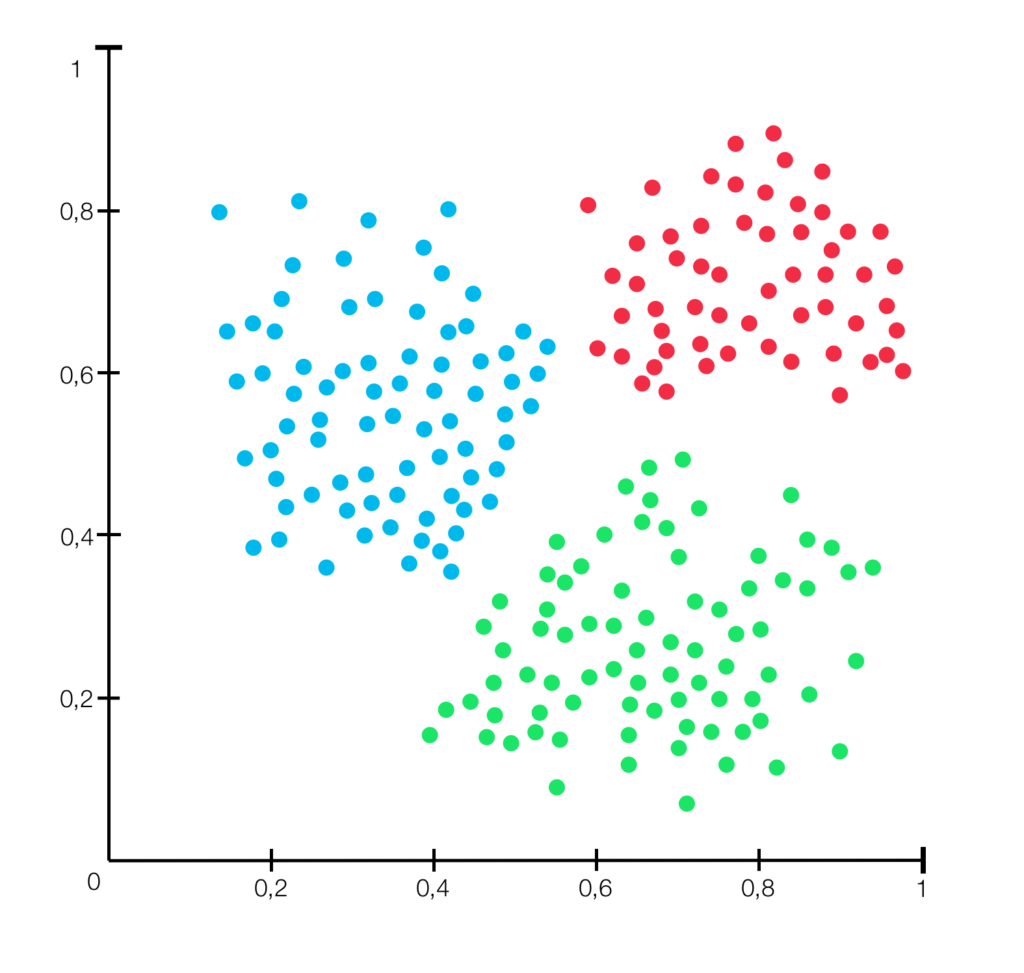
\includegraphics[scale=0.2]{cluster1.png}
\caption{Figura ilustrativa do agrupamento de clusters.}
\end{wrapfigure}

\quad Um \textbf{cluster} é um conjunto de objetos similares entre si e dissimilares em relação a objetos noutros clusters. A análise de clusters ou o seu conceito, é um procedimento humano normal, muitas vezes usado de forma inconsciente. \hyperlink{clusters}{\large$\bigskip^{[6][7]}$}
\par Muito cedo nas escolas, os alunos aprendem a classificar e agrupar, por exemplo distinguir entre gatos e cães, entre animais e planta, progredindo num refinamento de classificação que tem subjacente teorias de \textit{clustering}. A análise de clusters é usada em inúmeras aplicações, tais como no reconhecimento de padrões (\textit{machine learning}), processamento de imagem e pesquisa de mercado.

%Um \textbf{cluster} é um conjunto de objetos similares entre si dentro do mesmo cluster e dissimilares em relação a objetos noutros clusters. A análise de clusters ou o seu conceito, é um procedimento humano normal, muitas vezes usado de forma inconsciente. \hyperlink{clusters}{\large$\bigskip ^{[6][7]}$} \par\noindent Muito cedo nas escolas, nos primeiros anos de educação as crianças aprendem a classificar e agrupar, por exemplo distinguir entre gatos e cães, entre animais e plantas, progredindo num refinamento de classificação que tem subjacente teorias de\textit{clustering}. A análise de clusters tem sido usada em inúmeras aplicações, tais como reconhecimento de padrões na análise de dados, processamento de imagem e pesquisa de mercado.



\section{Clustering}
\begin{wrapfigure}{r}{0.4\textwidth}
\vspace{-2cm}
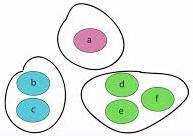
\includegraphics[scale=1.2]{clustering.png}
\caption{Clustering.}
\end{wrapfigure}

\quad O \textit{clustering} é o conjunto de técnicas de prospeção de dados, isto é, exames minuciosos e metódicos, que fazem agrupamentos automáticos de dados segundo o seu grau de semelhança. Normalmente o usuário do sistema deve escolher a priori o número de grupos a serem detetados. Alguns algoritmos mais sofisticados pedem apenas o número mínimo e outros tem a capacidade de subdividir um grupo em dois. Existem vários tipos de agrupamentos, mas o que será analisado com mais detalhe serão os \textbf{particionais}.

\subsection{Clustering na História}
\quad O primeiro registo publicado sobre um método de clustering foi feito em 1948, com o trabalho de \textit{SORENSEN} (1948) sobre o Método Hierárquico de Ligação Completa. Desde então mais de uma centena de algoritmos distintos de clustering já foram definidos. 


\section{Clusters Particionais}
\subsection{O que são?}
\quad Cluster particional define-se, especificamente, pelo facto de ao utilizar o agrupamento particional estar a dividir objetos de dados em subconjuntos sem sobrepor grupos, o que leva a que cada dado esteja exatamente num subconjunto.

\begin{figure}[h]
\centering
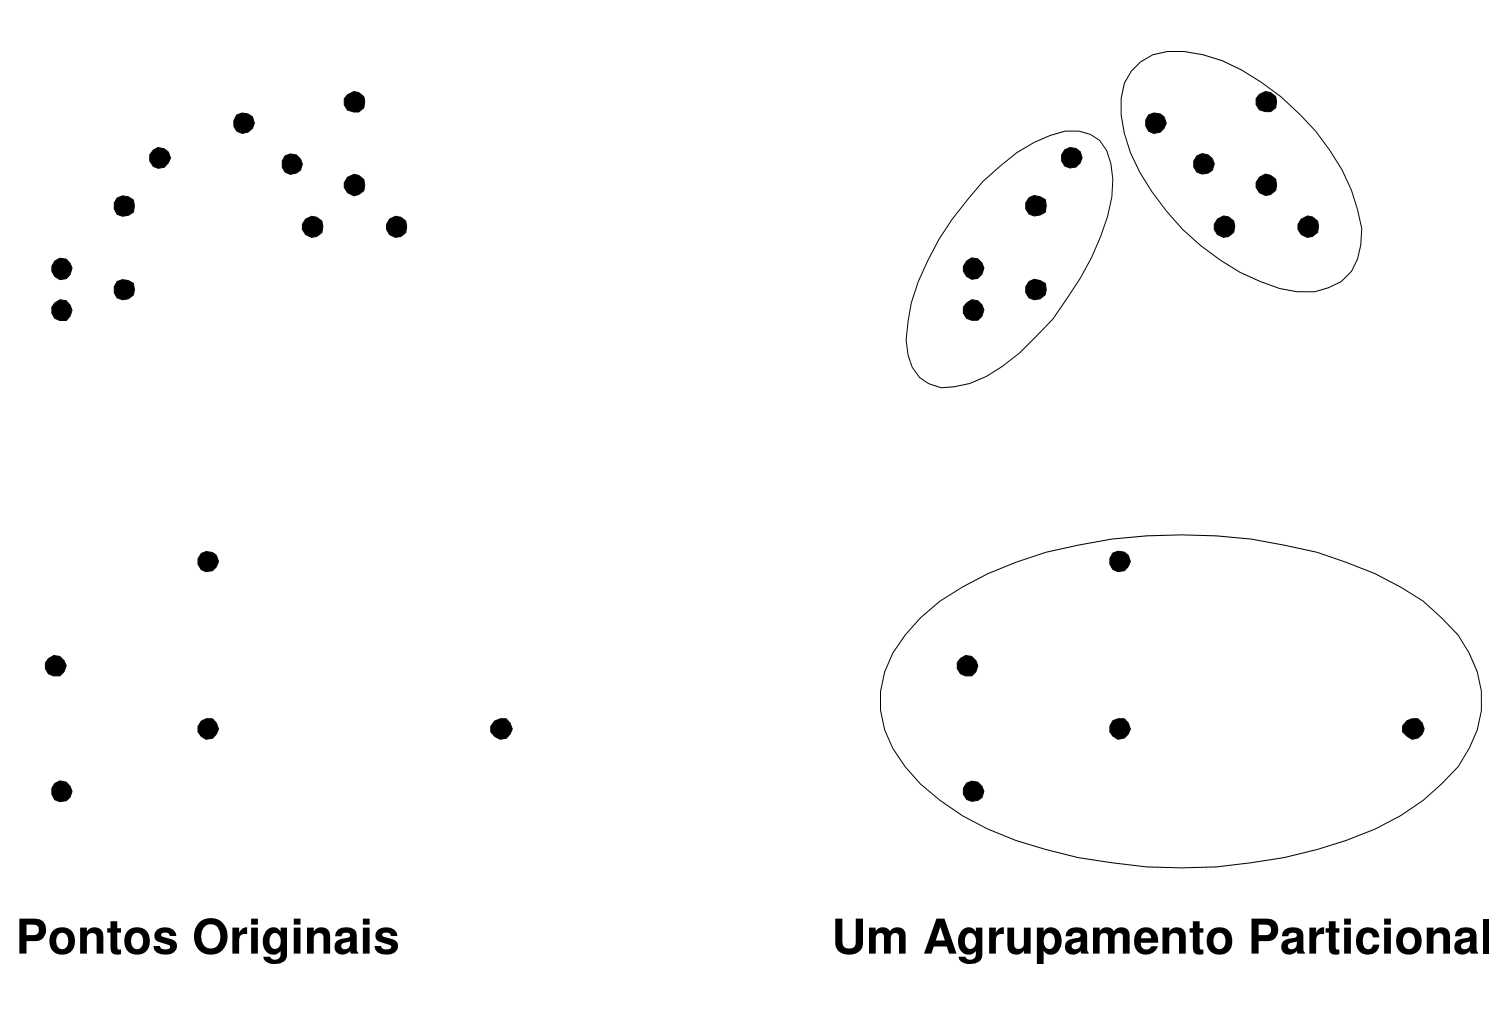
\includegraphics[scale=0.3]{cluster particional.png}
\caption{Cluster Particional}
\end{figure}







%---------------------------------------------------------
% Centróides
%---------------------------------------------------------


\chapter{Centróides}
\section{O que são?}
\quad Um \textbf{centróide} é o ponto que representa o \textit{centro} de todos os pontos pertencentes a um cluster.
No que diz respeito aos modelos centróides, a noção de similaridade deriva da proximidade dos pontos com o centróide do \textit{cluster}.\par
\par Além disso, os centróides são obtidos através de operações algébricas (somas e multiplicações por escalares) e, em regra, estes não pertencem à base de dados. Logo, são uma mera interpretação de resultados e que dependem maioritariamente da definição de proximidade entre dois objetos de estudo.

\section{Relação entre centróide e média}
\subsection{Semelhanças}
\quad ... a \textit{média} de um cluster é o mesmo que o centróide, contudo o termo \textbf{centróide} é mais preciso quando se estuda \textit{multivariate dada}, isto é, dados multivariados. 
\par Um centróide é ás vezes denominado de \textbf{centro de massa} ou  \textbf{barycenter}(centro de gravidade), baseado na sua interpretação física. Assim como a média, a localização do centróide \textbf{minimiza a \textit{sum-squared distance} entre os outros pontos}.

\subsection{Medóide} 
\quad Uma ideia semelhante é a de \textbf{medóide}, que é o ponto de dado que é \textit{menos parecido} de todos os outros pontos de dados. 
\par Ao contrário do centróide, a medóide tem de ser um dos pontos originais. 

\subsection{Diferenças}
\par Há, no entanto, uma diferença entre \textbf{distância de centróide} e \textbf{distância média} quando se comparam clusters. A distância de centróide entre dois quaisquer clusters A e B é simplesmente a distância entre o centróide de A e o centróide de B. Já a distância média é calculada encontrando-se a distância média entre todos os pares de pontos de cada cluster.

\begin{myequation}[!ht]
$$
	 \text{dist(}A,B\text{)} = \frac{\sum_{ij}\text{dist(}a_i,b_j\text{)}}{\#A \times \#B} , \quad \forall a_i \in A, b_j \in B $$

\caption{Métrica de Clusters: Distância média}
\vspace{0.5cm}
$$
	 \text{dist(}A,B\text{)} = \text{dist\Bigg(}\frac{\sum_{i} a_i}{\#A}\text{,}\frac{\sum_{i} b_i}{\#B}\text{\Bigg)} , \quad \forall a_i \in A, b_i \in B $$

\caption{Métrica de Clusters: Distância entre centróides}
\end{myequation}

Estes dois cálculos são duas métricas possíveis para calcular a distância entre dois clusters, mas existem mais métodos.\hyperlink{dist_clusters}{\large$\bigskip^{[8]}$}

\subsection{Exemplo}

\section{Como se determinam?}


%------------------------------------------------------------
%	Algoritmos
%-----------------------------------------------------------

\chapter{Os Algoritmos de Clusters Particionais}
O Cluster Particional tem dois algoritmos: o K-means e o K- medoids. Estes algoritmos tem as suas diferenças. Uma delas é o facto de K-means temos a soma máxima das distâncias, em K-medoids temos a soma mínima nas distancias.

\section{Representação dos Dados}

\begin{itemize}[leftmargin=0.375cm]
\item K representa o número e clusters
\item $(m^{1},...,m^{k},...,m^{K})$ K pontos distintos de D
\item $(x^{1},...,x^{n},...,x^{N})$ representa a base de dados
\item d representa uma função distância
\end{itemize}

\section{K-Means}
\subsection{O que é?}
\quad O \textit{K-Means} é um algoritmo de \textit{clustering} bastante comum e popular usado por numerosos investigadores em todo o mundo. Este tem por objetivo por em partes $n$ observações dentro de $k$ clusters, onde cada observação está dentro do cluster com que tem a média mais próxima, usando o Diagrama de Voronoi.
Nestes modelos, os números de clusters necessários no final ($n$) têm de ser mencionados com antecedência, o que torna importante o conhecimento prévio do conjunto de dados.
\par Na maioria das vezes, o método \textit{Elbow} é usado ou com a soma de erros quadrados (sse) ou  com a soma dos erros 
do cluster (wcss) (EXPLICAR O QUE CADA UM É!).

\subsection{Diagrama de Voronoi}
O diagrama de Voronoi relaciona-se com o algoritmo K-means pelo facto de que o diagrama é uma parte do conjunto de dados com alguns pontos centrais, que se denominam de centroides. Estes centroides não pertencem a base de dados, e um centroide é a localização (pode ser real ou imaginária) do centro de um cluster.
\subsection{Restrições}
Uma restrição que este algoritmo tem é o facto de apenas funcionar com atributos quantitativos, necessita de fazer operações algébricas, como somas e multiplicações por escalar, que dará origem uma matriz que é a “matriz da partição”. A nível de pontos que se encontram fora da curva, tem que se ter cuidado devido ao facto de os mesmos poderem facilmente influenciar o valor da média e levar a mesma a alterar-se.
\subsection{Determinação do K-Means}
\textbf{1º Passo:}
Temos de determinar os clusters que estão associados a M, e para isso temos de ter cuidado com os algoritmos fora do grupo, para não se influenciar a mesma e para isso podemos utilizar um número mediano.
	\begin{center}
	\ $ M=(m^{1},...,m^{k},...,m^{K})\rightarrow P=(P^{1},...,P^{k},...,P^{K})$
	\ $P^{k}=x^{i}\in D:d(x^{i},m^{k})< d(x^{i},m^{j}),j\in(1,...,k-1,k+1,...,K)$
	\end{center}	 
\textbf{2º Passo:}
Temos de determinar os novos centroides associados a P, pegando no primeiro conjunto de dados e fazer uma seleção aleatória de k pontos de dados para se verificar onde se encontra o centro.
	\begin{center}
	\ $ P=(p^{1},...,p^{k},...,p^{K})\rightarrow M=(m^{1},...,m^{k},...,m^{K})$
	\begin{myequation}[!ht]
$$ m^k = \frac{1}{|P^k|}\sum_{x \in P^k} x
	  $$
	 \caption{\small Fórmula do K-Means}

\end{myequation}
\end{center}
\textbf{3º Passo:}
Repetir os dois passos anteriores até se verificar que nenhum cluster muda de grupo.
 	\begin{center}
	\begin{figure}[h]
	\begin{subfigure}{.5\textwidth}
	\includegraphics[scale=0.4]{gráfico bem feito.png}
	\caption{Gráfico bem resolvido por K-Means}
	\end{subfigure}
	\begin{subfigure}{.5\textwidth}
	\includegraphics[scale=0.385]{gráfico mal feito.png}
	\caption{Gráfico mal resolvido por K-Means}
	\end{subfigure}
	\end{figure}
	\end{center}
	
	\newpage
\section{K-Medoids}
\subsection{O que é?}
idk

\section{Diferença entre K-Means e K-Medoids}
\subsection{A nível de técnica}
\quad O \textit{K-medoid} é uma técnica de cluster particional que trata de juntar dados dentro de um conjunto de n objetos em k agrupamentos, tendo em conta que k é conhecido a priori, o que exige que o programador deve especificar k antes de executar o algoritmo. Para a escolha de K temos dois métodos que podemos utilizar: \textbf{The Elbow Method} e o \textbf{The silhouette Method}. Já no \textit{k-means} o k é escolhido previamente. 
\subsection{A nível de sensibilidade}
\quad O \textit{K-medoid} lida melhor com os \textit{outliers} (pontos fora da curva) do que \textit{K-means}, é menos sensível a eles, porque minimiza a soma das diferenças contrariamente a \textit{k-means}, que maximiza.
\subsection{A nível de Centróide}
\quad O centro de \textit{k-medoids} não é o ponto médio mas sim um ponto real, porque é o objeto mais centralmente localizado do cluster, que como já referi, tem somas mínimas de distancia.
\subsection{A nível atributos}
\quad Os atributos de \textit{K-medoids} podem ser atributos quantitativos, tal como \textit{k-mean}, mas também podem ser atributos qualitativos, o que leva a que não exista uma necessidade e obrigação do uso de operações algébricas neste algoritmo. Estes atributos encontram-se representados na base de dados.


%----------------------------------------------------------------------------------------
%"The Elbow Method"
%----------------------------------------------------------------------------------------

\chapter{O Método Elbow}
\section{O que é?}
\quad Uma etapa fundamental para qualquer aprendizagem não-supervisionada é determinar o número ideal de clusters segundo os quais os dados podem ser agrupados: \textbf{K}.
\par O \textbf{The Elbow Method} é uma heurística, uma vez que, é um método criado para encontrar soluções sobre um problema, neste caso, para determinar o número ideal de clusters no \textit{k-means clustering}. Este método parcela o valor da função custo produzida pelos diferentes valores de \textbf{K}. Ora, isto só é possível, ignorando parte da informação com o objetivo de tornar a escolha mais fácil e rápida.
\par
Sendo assim, não há uma resposta universal para este problema já que o número ideal de \textit{clusters} é de alguma forma subjetivo e depende do método usado para medir as similaridades e os parâmetros usados para particionar. Portanto, em algumas situações, pode ser considerado ambíguo e pouco confiável. Nesse caso, é preferível utilizar-se outras abordagens para determinar o número de clusters.
\section{Como se aplica?}
\subsection{Pré-aplicação}
\quad
Numa fase inicial, criar um dendrograma, ou seja, um diagrama que organize as variáveis, agrupando-as de forma hierárquica ascendente - o que em termos gráficos se assemelha aos ramos de uma árvore.
\par 
Seguidamente, inspecionar o dendrograma produzido usando o cluster hierárquico para verificar se ele sugere um número específico de clusters. (Todavia, esta abordagem também é subjetiva.)
\par
Estes métodos, apresentados a seguir, incluem métodos diretos e teste estatístico:
\begin{itemize}[leftmargin=1cm]
\item \textbf{Métodos diretos}: consistem em otimizar um critério, como a somas de erros quadrados dentro do \textit{cluster} ou a média silhouette. Os métodos correspondentes são denominados métodos de \textit{Elbow} e silhouette, respetivamente.
\item \textbf{Métodos de teste estatístico}: consiste em comparar evidências contra hipóteses nulas. Um exemplo é a estatística de gap.\par
\end{itemize}
É importante referir ainda que, a ideia básica por detrás dos métodos de particionamento, como o \textit{k-means clustering}, é definir clusters de forma que a variação total intra-cluster, ou a soma total quadrada dentro do cluster (WSS), seja minimizada.\par
%----------------------------------------------------------------------------------------
\subsection{WCSS}
O código abaixo é uma maneira fácil de obter o valor wcss para diferentes números de clusters.\par
\begin{figure}[h]
  \centering
  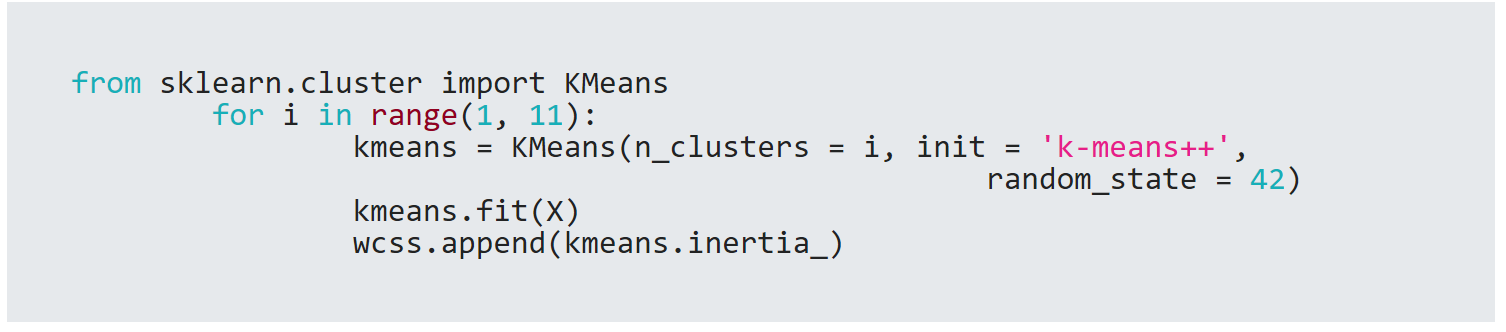
\includegraphics[scale=0.7]{1.png}
  \caption{Código para obtenção de valor wcss}   
  \label{fig:picture}
\end{figure}
\begin{figure}[b]
  \centering
  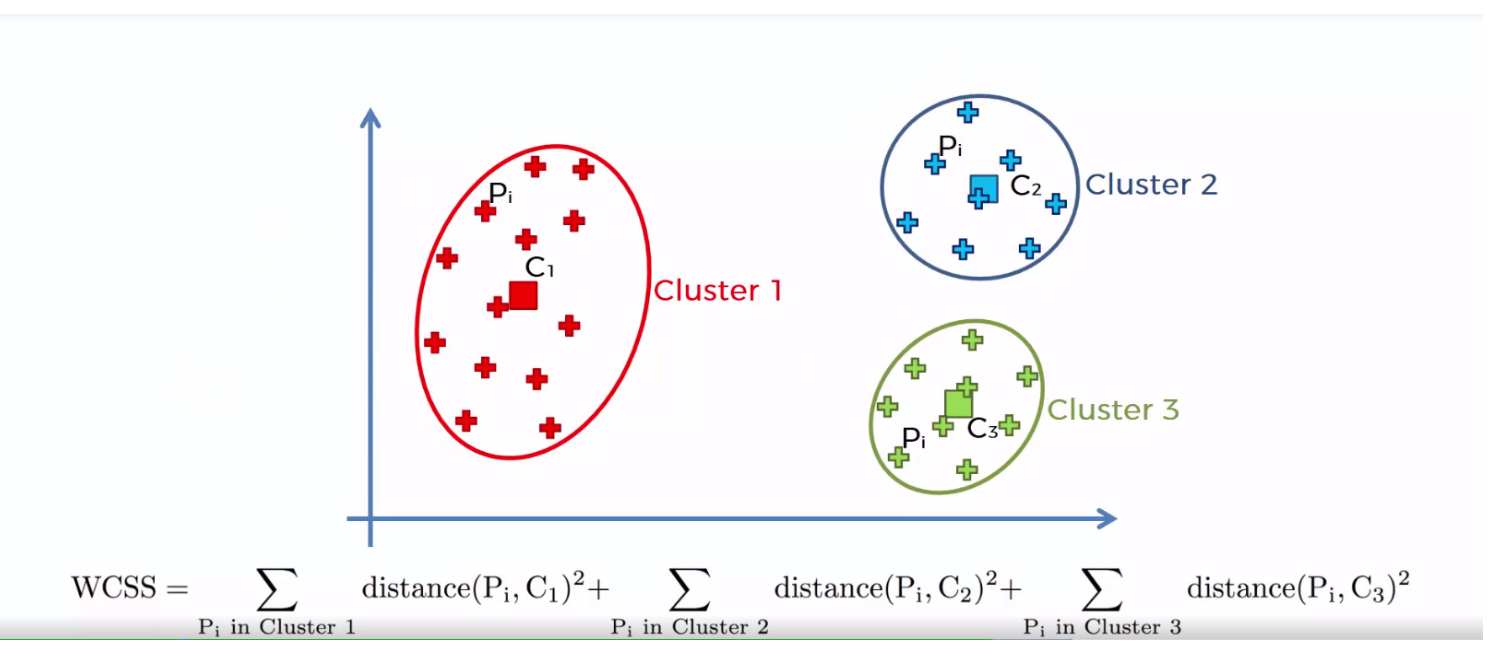
\includegraphics[scale=0.5]{2.png}
  \caption{Cálculo do valor wcss para três conjuntos de dados de \textit{cluster}}  
  \label{fig:picture}
\end{figure}
Assim como o nome sugere, \textbf{wcss} é o somatório da distância de cada cluster entre esses clusters específicos e cada um dos pontos contra o centróide do cluster.\par


%--------------------------------------------------
\subsection{Processos}
\quad O método de Elbow considera o WSS total como uma função do número de clusters: deve-se escolher um número de clusters para que a adição de outro cluster não melhore muito mais o WSS total.\par
O número ótimo de clusters pode ser obtido da seguinte forma:\par
\begin{enumerate}[leftmargin=2cm, align=left]
\item	Calcular o algoritmo de \textit{clustering}, por exemplo, \textit{k-means clustering}, para diferentes valores de \textit{k}. Por exemplo, variando \textit{k} de 1 a 10 clusters;\par
\item	Para cada \textit{k}, calcular a soma total quadrada (WSS) dentro do \textit{clusters};\par
\item	Fazer o gráfico (curva) de wws de acordo com o número de \textit{clusters k};\par
\item	A localização de uma curva, curva joelho, provavelmente, é uma curva com uma dobra acentuada, é geralmente considerada um indicador do número apropriado de \textit{clusters}.\par
\end{enumerate}
 
\begin{figure}[h!]
  \centering
  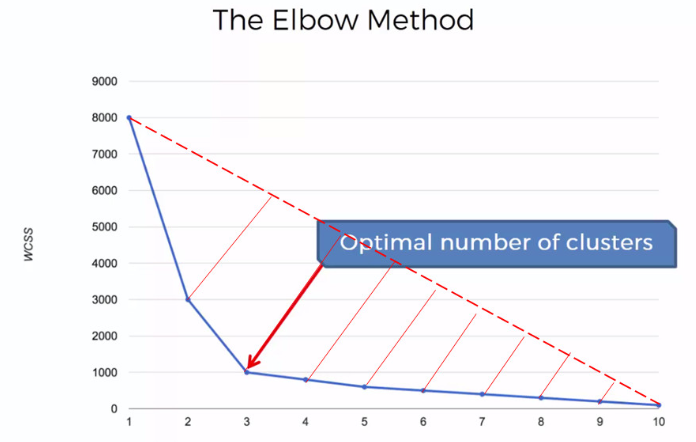
\includegraphics[scale=0.4]{3.png}
  \caption{Valor de wcss \textit{versus} número de \textit{clusters}}   
  \label{fig:picture}
\end{figure}

\par Uma alternativa é o método de \textit{silhouette} média (\textit{Kaufman e Rousseeuw} [1990]), que também pode ser usado com qualquer abordagem de \textit{clustering}.
%----------------------------------------------------------------------------------------

%----------------------------------------------------------------------------------------
%Exemplos
%----------------------------------------------------------------------------------------
\newpage
\chapter{Aplicações práticas}
\section{Exemplo 1}
\subsection{Como aplicar Clustering:}

Para aplicar o algoritmo, precisamos de primeiro criar alguns conjuntos aleatórios de pontos e distribui-los com algum espaçamento.

\bigskip
\begin{lstlisting}
points = make_blobs(n_samples=300, centers=4, cluster_std=0.60, random_state=0);
points.scatter(distance=1.5);
\end{lstlisting}

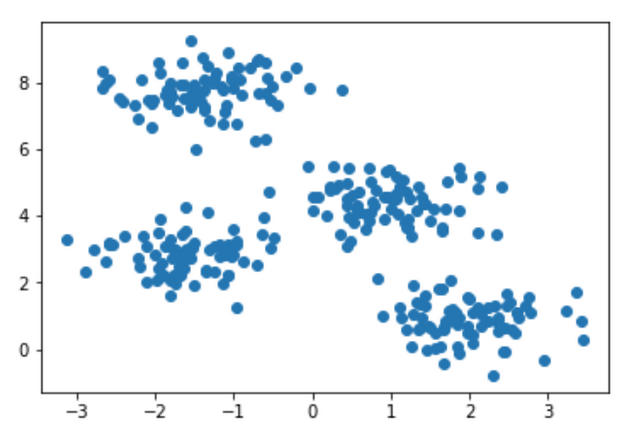
\includegraphics[scale=0.5]{ex1.png}

De seguida vamos aplicar kmeans aos nossos pontos. Vamos aplicar a função várias vezes, para numeros de clusters  desde 1 até 9 e vamos guardar o valor de WCSS de cada resultado.

\begin{lstlisting}
int wcss[10]; 

for(int i=1; i<10; i+=1) {
	kmeans = points.KMeans(n_clusters=i, init="k-means++", max_iter=300, n_init=10, random_state=0);
	wcss[i] = kmeans.getWCSS();
}
\end{lstlisting}


Com os falores de WCSS obtidos podemos gerar um gráfico que os relaciona com o respetivo numero de clusters.

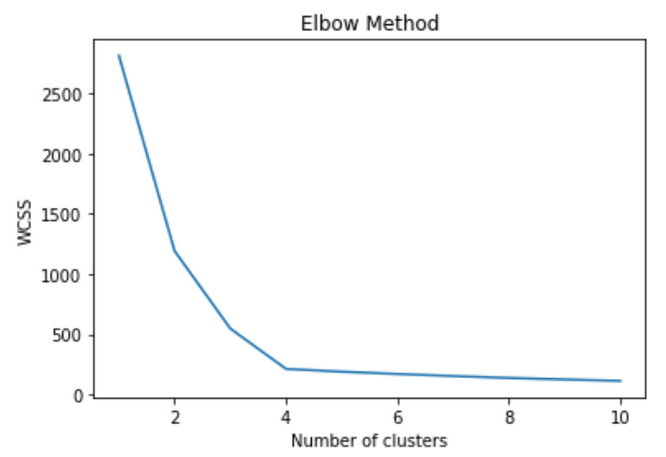
\includegraphics[scale=0.5]{ex2.png}

%-------------------------------------------------------
% Conclusão
%-------------------------------------------------------
\newpage
\chapter{Conlusões}
%-------------------------------------------------------
% Referências bibliográficas
%-------------------------------------------------------

\renewcommand\refname{Referências}

\begin{thebibliography}{9}
\bibitem{knuthwebsite} 
\textit{What is “Within cluster sum of squares by cluster” in K-means}\par
\UrlFont{\url{https://discuss.analyticsvidhya.com/t/what-is-within-cluster-
sum-of-squares-by-cluster-in-k-means/2706}}
\normalfont
\bibitem{knuthwebsite} 
\textit{Elbow Method},\par
\UrlFont{\url{https://www.scikit-yb.org/en/latest/api/cluster/elbow.html}}
\normalfont
\bibitem{knuthwebsite} 
\textit{Determining the optimal number of clusters},\par
\UrlFont{\url{https://www.datanovia.com/en/lessons/determining-the-optimal-
number-of-clusters-3-must-know-methods/\#elbow-method}}
\normalfont
\bibitem{knuthwebsite} 
\textit{Finding the optimal number of clusters for K-Means through Elbow
method using a mathematical approach compared to graphical approach},\par
\UrlFont{\url{https://www.linkedin.com/pulse/finding-optimal-number-clusters-k-means-through-
elbow-asanka-perera}}
\normalfont
\bibitem{einstein} 
Lachi, Ricardo Luís \& Rocha, Heloísa Vieira da. Fevereiro 2005.
\textit{Aspectos básicos de \textit{clustering}: conceitos e técnicas }. (Brasil).
\normalfont
\hypertarget{clusters}{
\bibitem{knuthwebsite}
\UrlFont{\url{https://www.maxwell.vrac.puc-rio.br/24787/24787_5.PDF}}
\bibitem{knuthwebsite}
\UrlFont{\url{http://www.dei.isep.ipp.pt/~paf/proj/Julho2003/Clustering.pdf}}}
\normalfont
\hypertarget{dist_clusters}{
\bibitem{einstein}
\textit{Hierarchical Clustering 3: single-link vs. complete-link}
\UrlFont{\url{https://www.youtube.com/watch?v=VMyXc3SiEqs}}
}
\end{thebibliography}

\end{document}